\documentclass[12pt]{article}

\usepackage{amsmath,amsthm,amssymb}
\usepackage{tikz}

\newcommand{\A}{\mathcal{A}}
\newcommand{\G}{\mathcal{G}}
\renewcommand{\P}{\mathfrak{A}}
\newcommand{\C}{\mathfrak{C}}
\newcommand{\Z}{\mathbb{Z}}
\newcommand{\Q}{\mathbb{Q}}
\newcommand{\2}{\textbf{2}}
\newcommand{\Am}{\textbf{A}}
\newcommand{\del}{\partial}
\renewcommand{\v}{\bar{v}}
\newcommand{\T}{\mathcal{T}}

\newtheorem{thm}{Theorem}

\title{Extensions of Abelian Automata Groups}
\author{Chris Grossack}

\begin{document}
\maketitle

\section{Background}

\subsection{Mealy Automata}
Recall a \textbf{Mealy Automaton} is a combinatorial object which defines
functions from $\Sigma^* \to \Sigma^*$ for some alphabet $\Sigma$
(As usual, $\Sigma^*$ denotes the free monoid generated by $\Sigma$).
In the special case each of these functions is invertible, we say the
Automaton is an \textbf{Invertible Transducer}. For our purposes, 
a Mealey Automaton is a tuple 
$\A = (S, \Sigma, \delta)$
where $S$ is the \textbf{State Set}, $\Sigma$ is the \textbf{Alphabet},
and $\delta~:~S \times \Sigma \to S \times \Sigma$ is the
\textbf{transition function}.

Given a state $s \in S$, we can treat it is a function 
$\underline{s} : \Sigma^* \to \Sigma^*$ by 

\begin{align*}
  \underline{s}(\varepsilon) &= \varepsilon\\
  \underline{s}(ax)       &= a' \underline{s'}(x) 
  ~~~(\text{where } (s', a') = \delta(s,a))
\end{align*}
Where juxtaposition is concatenation, and $\varepsilon$ is
the identity in $\Sigma^*$.
Clearly we could treat $\underline{s}$ as a function on $\Sigma^\omega$ 
instead, and in fact we occasionally will, however we will be 
clear when doing so.

In general, one can look at the semigroup generated by an automaton $\A$,
namely the semigroup generated by $\{ \underline{s}~|~s \in S \}$.
For the rest of the paper, however, we will restrict ourselves to the
invertible case, and will consider $\G(\A)$, the group generated by 
$\{ \underline{s}~|~s \in S \}$ instead.

As an example, consider the automaton (shown below)
$\A = (\{ \alpha, \tau \}, \2, \delta)$
with 
\begin{align*}
  \delta(\alpha,0) &= (\alpha,1)\\
  \delta(\alpha,1) &= (\tau,0)\\
  \delta(\tau,0)   &= (\alpha,0)\\
  \delta(\tau,1)   &= (\tau,1)
\end{align*}

TODO: is this correct?

\begin{center}
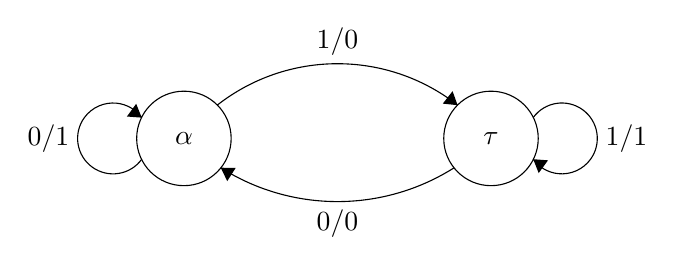
\begin{tikzpicture}[scale=0.2]
\tikzstyle{every node}+=[inner sep=0pt]
\draw [black] (15.8,-29.2) circle (3);
\draw (15.8,-29.2) node {$\alpha$};
\draw [black] (35.3,-29.2) circle (3);
\draw (35.3,-29.2) node {$\tau$};
\draw [black] (13.12,-30.523) arc (-36:-324:2.25);
\draw (8.55,-29.2) node [left] {$0/1$};
\fill [black] (13.12,-27.88) -- (12.77,-27) -- (12.18,-27.81);
\draw [black] (17.918,-27.085) arc (128.02449:51.97551:12.39);
\fill [black] (33.18,-27.09) -- (32.86,-26.2) -- (32.24,-26.99);
\draw (25.55,-23.96) node [above] {$1/0$};
\draw [black] (37.98,-27.877) arc (144:-144:2.25);
\draw (42.55,-29.2) node [right] {$1/1$};
\fill [black] (37.98,-30.52) -- (38.33,-31.4) -- (38.92,-30.59);
\draw [black] (32.957,-31.065) arc (-57.68311:-122.31689:13.856);
\fill [black] (18.14,-31.06) -- (18.55,-31.91) -- (19.09,-31.07);
\draw (25.55,-33.71) node [below] {$0/0$};
\end{tikzpicture}
\end{center}

Somewhat surprisingly, $\G(\A)$ is the lamplighter group, $\Z/2\Z \wr \Z$

\subsection{Abelian Automata}
We restrict ourselves to the case where $\G(\A)$ is abelian, 
and use methods of Nekrashevich and Sidki to characterize these groups.
Further, we can take some combinatorial information from our Mealy 
Automaton, and push it into the group theoretic world. This will give
rise to much of the interesting structure of these groups, since
$\G(\A)$ is abelian if and only if it is either free abelian or 
boolean.

It is well known that in an Invertible Transducer, each $\delta(s,-)$
is a permutation of $\Sigma$. Since our automata will be over the alphabet
\2, this means every state either flips its input 
(in which case it is called an \textbf{Odd} or \textbf{Toggle State}), 
or does not
(in which case it is called an \textbf{Even} or \textbf{Copy State}).
We extend these definitions to the entire group, and say $f \in \G(\A)$ 
is odd iff it flips the first bit of its input.

Further, we define $\del_0, \del_1 : \G(\A) \to \G(\A)$ by 
$\del_i \underline{s} = \underline{\delta(s,i)}$\ldots

TODO: better way to define this?

It is a theorem by Sutner that $\G(\A)$ is abelian iff for 
even states $\del_0 f - \del_1 f = I$ and for odd states
$\del_0 f - \del_1 f = \gamma$, where $\gamma$ is independent
of $f$. Here we write $I$ for the identity element of our group,
and we use additive notation since our groups are abelian.

Further, the case $\gamma = I$ corresponds precisely to the $\G(\A)$
being boolean.

We now restrict ourselves further to the case where $\G(\A)$ is 
free abelian, that is to say $\G(\A) \cong \Z^m$ for some $m$,
and $\gamma \not = I$.
If $\varphi$ witnesses this isomorphism, then $\varphi(f)$ has odd
first component iff $f$ is odd. To that end, we call a vector $\v$ odd
if its first component is odd, and even otherwise.

A theorem by Nekrashevich and Sidki tells us that

\begin{thm}
  There is a matrix $\Am$ associated to each automaton 
  (though multiple automata may share a matrix, as we will soon see)
  such that for any odd vector $\bar{e}$ 
  \[ \del_0 f = \Am (\varphi(f) - e) \] and
  \[ \del_1 f = \Am (\varphi(f) + e) \]
  Futher, $\Am$ is a contraction (all its complex eigenvalues have norm $<1$),
  and $\Am$ has irreducible characteristic polynomial 
  $\chi(x) = x^m + \frac{1}{2}g(x)$, 
  where $g \in \Z[x]$ has constant term $\pm 1$
\end{thm}

To that end, we can define the \textbf{Complete Automaton} 
$\mathfrak{C}(\Am, \bar{e})$ as the Mealy machine whose state set is all of
$\Z^m$, and whose transitions are given by the above formulas.

Notice that we can take any state $f \in \mathfrak{C}(\Am, \bar{e})$, 
and close $\{ f \}$ under residuation.
Further, since $\Am$ is a contraction, the resulting closure will be finite.
We call this machine $\A_f$, and recognize $\G(\A_f)$ is a subgroup of 
$\G(\mathfrak{C}(\Am, \bar{e}))$.

The free parameter $\bar{e}$ seems confusing at first. Particularly 
when one tries to understand how it effects the $\A_f$ which live in
$\mathfrak{C}(\Am, \bar{e})$. We will show later that every abelian automaton
lives in $\mathfrak{C}(\Am, \bar{e})$ for infinitely many $\bar{e}$, and
further we will characterize exactly which $\bar{e}$ these are, and for which
$f$ is $\A_f \subseteq \mathfrak{C}(\Am, \bar{e})$ the desired automaton.

To that end, we will say that a function $f$ is \textbf{Located at} 
$\v \in \mathfrak{C}(\Am, \bar{e})$ iff some isomorphism $\varphi$ sends 
$f$ to $\v$. We make an analogous definition for an entire automaton $\A$
being \textbf{Located at} $f$ if 
$\A = \A_f \subseteq \mathfrak{C}(\Am, \bar{e})$

\subsection{Principal Automata}

\section{Group Extensions}
Going forward, $\G$ will denote $\G(\P)$ for some principal machine $\P$.

In the case of interest, $\G \cong \Z^m$. Further, $\del_0$ extends to 
a $\frac{1}{2}$-Integral matrix $\Am$ of irreducible character. Then
$\G$ admits representation as a $\Z[x]$ module where 
$x \cdot \v = \Am^{-1}\v$, extended linearly.
Further, since $\Am$ has irreducible character (in $\Z$ and in $\Q$), 
so does $\Am^{-1}$. Thus this module is cyclic, 
and generated by $\bar{e_1} = \delta$.

Clearly $\text{End}_{\G}$, the ring of module endomorphisms of $\G$, 
is isomorphic to $\Z[x]/(\chi^*)$, 
where $\chi^*$ is the characteristic polynomial of $\Am^{-1}$.
Now for some $p \in \text{End}_{\G}$ we consider
$p \cdot \G = \Z^m$, equipped with
$\del_0 \v = \Am (\v - p \cdot \bar{e_1})$, and 
$\del_1 \v = \Am (\v + p \cdot \bar{e_1})$
(thus we require $p$ have odd constant term).

For reasons which will soon become clear, we call $p \cdot \G$ the
\textbf{Group Extension} of $\G$ by $p$.

To justify this nomenclature, we first notice 
$\G \hookrightarrow p \cdot \G$ for all $p$ by the
homomorphism $\v \mapsto p \cdot \v$. 
Further, we recognize that if $p$ is not a unit in $\text{End}_{\G}$, 
this homomorphism is \emph{not} surjective. 
That is to say $\G$ is a proper subgroup of $p \cdot \G$.
\textbf{Note:} It \emph{is} the case that $\G \cong \Z^m \cong p \cdot \G$. 

Every function $f \in \G$ is also an element of $p \cdot \G$. 
If $f \in \G$ is located at $\v$, then $f \in p \cdot \G$ is located
at $p \cdot \v$. In fact, this is true in a more general sense:

\begin{thm}
  If $mp = q$, then $p \cdot \G \hookrightarrow q \cdot \G$, 
  with a canonical injection $\phi_m~:~\v \mapsto m \cdot \v$. 
  In particular, if $m$ is a unit, then $p \cdot \G \cong q \cdot \G$.
\end{thm}

\begin{proof}
  Let $mp = q$, $f \in p \cdot \G$ located at $\v$.
  Consider $f' \in q \cdot \G$ located at $m \cdot \v$.

  First note $f$ and $f'$ have the same parity, since 
  $m$ has odd constant term, and so $\v$ and $m \cdot \v$
  have the same parity. Now, consider the residuals of $f$ and $f'$. 
  
  If $f$ is even, then 
  \[ \del_0 f' = \Am (m \cdot \v) = m \cdot \Am \v = m \cdot \del_0 f \]

  If $f$ is odd, then
  \[ \del_0 f' = \Am (m \cdot \v - q \cdot \bar{e_1}) 
               = m \cdot \Am (\v - p \cdot \bar{e_1})
               = m \cdot \del_0 f \]

  A similar argument shows $\del_1 f' = m \cdot \del_1 f$
\end{proof}

\section{Fractional Elements}
So for $p \cdot \G$ we know exactly how vectors of the form $p \cdot \v$
behave as functions: They are exactly the functions present in $\G$.
However there are plenty of vectors which do not have the above form. 
How do they behave? We call such vectors (and their corresponding functions)
\textbf{Fractional}, due to the following observation.

Consider $3 \cdot \G$. What does $\bar{e_1}$ do as a function?
Well, $3\bar{e_1}$ should do the same function as $\delta$, and so
$\bar{e_1}$ should behave like ``$\frac{1}{3}\delta$'', and in fact it does.

In general, $\v \in p \cdot \G$ behaves like $p^{-1} \cdot \v \in \G$,
(where $p^{-1}$ comes from $\Q[x]$ and so $p^{-1} \cdot \v \in \Q^m$)
and so Group Extensions give us access to fractional functions from 
our base group $\G$.

\begin{thm}
  $\forall p \in Z[x]$ with odd constant term,\\
  $\{ p^{-1} \cdot \v~|~\v \in \Z^m \} (\leq \Q^m) \cong p \cdot \G$.\\
  Further, this isomorphism respects $\del_0$ and $\del_1$.
\end{thm}

\begin{proof}
  Let $p^{-1} \cdot \Z^m = \{ p^{-1} \cdot \v~|~\v \in \Z^m \}$\\
  Consider $\varphi~:~p^{-1} \cdot \Z^m \to p \cdot \G$ by
  $\varphi(p^{-1} \cdot \v) = \v$.\\
  $\varphi$ is clearly bijective, and is a homomorphism since:
  \begin{align*}
       \varphi(p^{-1} \cdot \v_1 + p^{-1} \cdot \v_2) 
    &= \varphi(p^{-1} \cdot (\v_1 + \v_2))\\
    &= \v_1 + \v_2\\
    &= \varphi(p^{-1} \cdot \v_1) + \varphi(p^{-1} \cdot \v_2) 
  \end{align*}

  Further, if $\v$ is even, then:

  \begin{align*}
       \varphi(\del_0 p^{-1} \cdot \v)
    &= \varphi(\Am p^{-1} \cdot \v)\\
    &= \varphi(p^{-1} \cdot \Am \v)\\
    &= \Am \v\\
    &= \del_0 \varphi(p^{-1} \cdot \v)
  \end{align*}

  If $\v$ is odd, then: 

  \begin{align*}
       \varphi(\del_0 p^{-1} \cdot \v)
    &= \varphi(\Am (p^{-1} \cdot \v - \bar{e_1}))\\
    &= \varphi(p^{-1} \cdot \Am (\v - p \cdot \bar{e_1}))\\
    &= \Am (\v - p \cdot \bar{e_1})\\
    &= \del_0 \varphi(p^{-1} \cdot \v)
  \end{align*}

  The $\del_1$ proof is similar, and has been omitted.
\end{proof}

Thus we can view functions in $p \cdot \G$ as fractions of functions in $\G$.
It is a natural question to ask which fractions are attainable in this way.

Clearly, for any $f \in \G$, we can attain $\frac{1}{k} f$ for any odd $k$.
However, even fractions are unattainable, even in limiting cases. 
This is clear, since $\frac{1}{2}\delta$, for instance, must 
when applied twice, flip the first bit of the input. But it must itself
be even or odd. In either case, $2 \frac{1}{2} \delta$ does not flip the 
first bit, a contradiction.

\section{Characterizing Automata}
Every strongly connected automaton $\A$ lives in $p \cdot \G$ where 
$\G$ is the principal group associated to $\A$ and $p$ is a polynomial. 
Further, $\A$ can always be anchored with an odd state at $\bar{e_1}$. 
Thus, the study of Group Extensions is sufficient to study all abelian automata.

\begin{thm}
  Every strongly connected abelian automaton $\A$ can be anchored with an 
  odd state at $\bar{e_1}$ in $p \cdot \G$ as above.
\end{thm}

\begin{proof}
  Let $f$ be an odd state in $\A$. Then $f_0$ and $f_1$ are distinct
  and both have paths to $f$ by strongly connectedness. Thus we have two
  distinct cycles $c_0$ and $c_1$ from $f$ to $f$ in $\A$.
  Each of these cycles gives rise to a matrix equation 
  $\v_f = g_0(\v_f,\bar{e}) = g_1(\v_f,\bar{e})$ corresponding to following
  the path in $\Z^m$ (with unknown residuation vector $\bar{e}$). 
  Then $(g_0 - g_1)(\v_f, \bar{e}) = \bar{0}$ and we can solve for 
  $\bar{e}$ in terms of $\v_f$.

  Choosing $\v_f = \bar{e_1}$ gives a value for the residuation vector $e$,
  which (by cyclicity) gives a polynomial $p_e$ 
  such that $p_e \cdot \bar{e_1} = e$. Then, by construction, $\A$ is 
  a subautomaton of $p_e \cdot \G$, and is anchored with $f$ at $\bar{e_1}$.
  As desired.
\end{proof}

\section{Characterizing Orbits}

Recall an \textbf{Orbit} of $f \in \G(\A)$ at $u \in \2^{\omega}$
is $\{ f^t u | t \in \Z \}$, or, additively, $\{ tf u | t \in \Z \}$.
It is a reasonable question to wonder what these orbits look like
for an arbitrary automaton?

By the above theorem, it suffices to consider $f \in p \cdot \G$
for some principal group $\G$. Fix such a group.

We begin with a useful lemma

\begin{thm}
  $x^n \cdot \delta (u0v) = u1v$ (where $|u| = n$)
\end{thm}

\begin{proof}
  If $n=0$ the theorem is clear, since 
  $\delta 0v = 1 (\del_0 \delta v) = 1 (I v) = 1v$

  Further by induction, 
  $x^{n+1} \cdot \delta (u_0u0v) = 
  \Am^{-1} (x^n \cdot \delta) (u_0u0v) =
  u_0 (x^n \cdot \delta) (u0v) =
  u_0u1v$
\end{proof}

We will first prove the result in the finite case.

\begin{thm}
  For every word $u \in \2^n$, there exists a unique function
  (mod $Stab(0^n)$) $f$ such that $f 0^n = u$.
\end{thm}

\begin{proof}
  The existance of such a function is a direct consequence of the lemma,
  and is given by $\sum_{i=0}^{n-1} u_i x^i \delta$.
  Uniqueness mod $Stab(0^n)$ is immediate from basic group theory.
\end{proof}

Denote this function by $\langle u \rangle$. 

\begin{thm}
  The orbit of $f$ at $u$ is given by the line $\Z f + \langle u \rangle$
\end{thm}

\begin{proof}
  Let $w = tf u$. Then $\langle w \rangle$ sends $0^n$ to $w$, 
  but so does $tf + \langle u \rangle$. By uniqueness, then,
  $\langle w \rangle = tf + \langle u \rangle$ and the theorem follows.
\end{proof}

Note that this argument works in the infinite case as well, provided 
we have a suitable definition of $\langle u \rangle$ for $u \in \2^\omega$.
For cardinality reasons, we clearly cannot send $0^\omega$ to any $u$.
Below we will characterize exactly those $u$ for which a $\langle u \rangle$
exists.

\begin{thm}
  For $u \in \2^\omega$, $\langle u \rangle$ exists in some group extension
  iff $u$ is ultimately periodic.
\end{thm}

\begin{proof}
  Since every function $f \in p \cdot \G$ eventualy residuates into a 
  strongly connected component, $f 0^\omega$ is ultimately periodic for
  every such $f$.

  Further, if we have an ultimately periodic string $u = tv^*$, then
  $\sum_{i=0}^{\infty} u_i x^i \delta$ works if it exists. Further,
  it exists, since:

  \begin{align*}
    \sum_{i=0}^{\infty} u_i x^i \delta 
    &= \sum_{i=0}^{|t|} t_i x^i \delta 
        + \sum_{i=|t|}^{\infty} v^*_i x^i \delta\\
    &= \sum_{i=0}^{|t|} t_i x^i \delta 
        + x^{|t|} \sum_{i=0}^{\infty} v^*_i x^i \delta\\
    &= \sum_{i=0}^{|t|} t_i x^i \delta 
         + x^{|t|} \frac{\sum_{i=0}^{|v|} v_i x^i \delta}{1 - x^{|v|}}\\
    &= \left ( 
        \sum_{i=0}^{|t|} t_i x^i
        + x^{|t|} \frac{\sum_{i=0}^{|v|} v_i x^i}{1 - x^{|v|}}
       \right ) \cdot \delta\\
    &= \frac%
        {%
          1 - x^{|v|} \sum_{i=0}^{|t|} t_i x^i + 
          x^{|t|} \sum_{i=0}^{|v|} v_i x^i
        }
        {1 - x^{|v|}}
       \cdot \delta\\
    &= \frac{q}{1 - x^{|v|}} \cdot \delta
  \end{align*}

  Finally, this sum is convergent in the cantor topology, since 
  for each $N \geq 0$, for all $n \geq N$, the $nth$ partial sums 
  agree on the first $N$ bits of the string.

  Thus, this sum is equal to $q \cdot \delta \in 1 - x^{|v|} \cdot \G$.
\end{proof}

For ultimately periodic strings $u \in \2^\omega$, $f$ orbits
of $u$ correspond to lines $\Z f + \langle u \rangle$.
\end{document}
